\section{Überwachtes Lernen (supervised learning)}
	\begin{itemize}
		\item gegeben eine Anzahl an Trainingsdaten (Eingaben, Sollausgaben)
		\item \textbf{Ziel:} finde Modell für die Daten
		\item \textbf{Ziel:} Generalisierung (Exploitation)
		\item verschieden Möglichkeiten für \textbf{Exploitation}
		\begin{itemize}
			\item \textbf{deterministisch}: berechne neue Ausgabe für neue Eingabe
			\item \textbf{probabilistisch}: erzeuge zufällige Ausgabe für neue Eingabe mit gelernter Wahrscheinlichkeitsverteilung (predictive distribution)
		\end{itemize}
	\end{itemize}
	\subsection{Regression (Deterministisch)}
	\subsubsection{Datenmodell}
	\begin{itemize}
		\item Polynom vom Grad M
		\item \textbf{Annahmen:}
		\vspace*{-3pt}
		\begin{itemize}[$\hookrightarrow$]
			\leftskip15pt
			\item Form des Modells: Polynom
			\item Grad des Polynoms
			\begin{itemize}[$\hookrightarrow$]
				\leftskip15pt
				\item bestimmt Komplexität des Modells
				\item bestimmt die Anzahl der Parameter
			\end{itemize}
		\end{itemize}
	\end{itemize}
	\subsubsection{Parameteroptimierung}
	\begin{itemize}
		\item Summe der quadratischen Fehler: 
		\begin{equation*}
			E(\pmb{w}) = \frac{1}{2} \sum_{n=1}^{N}(y(x_n, \pmb{w})-t_n)^2
		\end{equation*}
		\item \textbf{Annahmen:}\vspace*{-3pt}
		\begin{enumerate}[$\hookrightarrow$]
			\leftskip10pt
			\item quadratische Fehlerfunktion
			\item \dq gute\dq Parameter für das Modell finden
		\end{enumerate}
		\item Betrachte $E(\pmb{w})$ als Funktion der Parameter $\pmb{w}$
		\item \textbf{Minimiere} quadratischen Fehler bezüglich $\pmb{w}$
		\item wir erhalten durch Einsetzen der Trainingsdaten den \textbf{Trainingsfehler}
		\item Danach: teste mit Daten, die nicht zum Lernen verwendet wurden, wir erhalten den \textbf{Testfehler}\vspace*{-5pt}
		\begin{enumerate}[$\hookrightarrow$]
			\leftskip10pt
			\item \textbf{Ziel:} Minimiere den Testfehler
		\end{enumerate}
	\end{itemize}
	\textbf{Problem:} Finden der richtigen Modellkomplexität.
	\begin{itemize}
		\item Fehlerminimierung allein funktioniert nicht\vspace*{-3pt}
		\begin{enumerate}[$\hookrightarrow$]
			\leftskip10pt
			\item $E(\pmb{w})=0$ ist bei verrauschten Daten unerwünscht
			\item ist das Modell zu komplex (zu viele freie Parameter), dann kann es das Rauschen lernen $E(\pmb{w})<<1$
			\item wenn Rauschen gelernt ist, dann ist die Generalisierung schlecht $\Rightarrow$ \textbf{Overfitting}
		\end{enumerate}
		\item $E_{RMS}$ zeigt Overfitting an
		\begin{equation*}
			E_{RMS}=\sqrt{2E(\pmb{w^*})/N}
		\end{equation*}
	\end{itemize}
	Maßnahmen gegen Overfitting:\vspace*{-5pt}
	\begin{enumerate}[$\hookrightarrow$]
		\leftskip10pt
		\item Modellselektion
		\item verändere \#Daten relativ zu \#Parameter
		\item stelle zusätzliche Bedingungen an die Parameter $\Rightarrow$ \textbf{Regularisierung}
	\end{enumerate}
	\textbf{Regularisierung} (hier):
	\begin{itemize}
		\item verbiete große Koeffizientenwerte\vspace*{-5pt}
		\begin{enumerate}[$\hookrightarrow$]
			\leftskip10pt
			\item beugt Oszillation vor (Bias!)
			\item macht die gelernte Funktion glatter (Bias!)
		\end{enumerate}
	\end{itemize}
	Regularisierung durch Bestrafung großer Koeffizienten:
	\begin{equation*}
		\tilde{E}(\pmb{w})=\frac{1}{2} \sum_{n=1}^{N}(y(x_n, \pmb{w})-t_n)^2+\underbrace{\frac{\lambda}{2}\left\Vert \pmb{w}\right\Vert^2}_{\mathclap{\substack{\text{Regularisierungsterm} \\ \text{$\lambda$ = wie wichtig ist Regularisierung}}}}
	\end{equation*}
	\begin{figure}[ht]
		\centering
		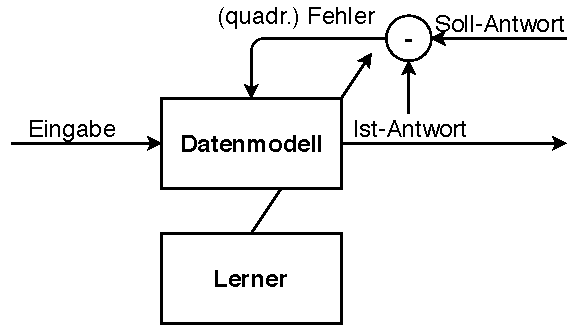
\includegraphics[width=.8\textwidth]{img/supervisedLearning}
		\caption{Vorgehensweise beim überwachten Lernen}
		\label{deployment}
	\end{figure}\\
	\subsection{Regression (Probabilistisch)}
	\subsubsection*{Modellierung durch Likelihood}
	\begin{itemize}
		\item für gegebenes parametrisiertes Datenmodell $y(x, \pmb{w})$
		\item \textbf{Likelihood} = bedingte Wahrscheinlichkeit eine Ausgabe $t$ bei gegebenen Parametern $\pmb{w}, \beta$ und Eingabe $x_0$ zu erhalten: $p(t\vert x_0, \pmb{w}, \beta)$.\vspace*{-3pt}
		\begin{enumerate}[$\hookrightarrow$]
			\leftskip10pt
			\item ist nach Annahme gaußverteilt mit Mittelwert $y(x_0, \pmb{w})$ und Varianz $\beta^{-1}=\sigma^2$ (1-dim. Fall):
			\begin{equation*}
				p(t\vert x_0, \pmb{w}, \beta) = N(t\vert y(x_0,\pmb{w}), \sigma^2)
			\end{equation*}
			\item $\beta$ heißt Präzision
			\item multidimensional:
			\begin{equation*}
				p(\pmb{t}\vert \pmb{x_0}, \pmb{w}, \Sigma^{-1}) = N(\pmb{t}\vert \pmb{y}(\pmb{x_0},\pmb{w}), \Sigma^{-1})
			\end{equation*}
		\end{enumerate}
	\end{itemize}
	\subsubsection{Zugrundeliegende Annahmen}
	\begin{itemize}
		\item es gibt nur einen Datensatz
		\item es gibt einen \dq wahren, idealen\dq Satz Modellparameter
		\item $\pmb{w_{ML}}$, $\beta_{ML}$ sind gute Approximationen
		\item Modellierung der Unsicherheit durch Störung resultiert in Verteilung
		\item Daten sind endlich und zufällig
		\item damit sind $\pmb{w_{ML}}$, $\beta_{ML}$ ebenfalls datenabhängig zufällig
		\item Unsicherheit in der Wahl des Datensatzes ist (noch) nicht modelliert	
	\end{itemize}
	\subsubsection{Von der Messung zur Wahrscheinlichkeit}
	\begin{itemize}
		\item für gegebenes parametrisiertes Datenmodell $y(x, \pmb{w})$ und gegebene Sollausgabe $t$
		\begin{equation*}
			t = y(x, \pmb{w}) + \underbrace{N(0, \beta^{-1})}_\text{Rauschen}
			\Leftrightarrow t - y(x, \pmb{w}) \sim N(0, \beta^{-1})
			\Leftrightarrow t \sim N(y(x, \pmb{w}), \beta^{-1})
		\end{equation*}
		\item \textbf{Datenmodell:} Normalverteilung um das Modell $y(x, \pmb{w})$ mit Eingabe $x$ und Parametern $\pmb{w}$
	\end{itemize}
	\subsubsection{Likelihood für alle Daten (Data-Likelihood)}
	\textbf{Annahme:} Daten unabhängig von einander erzeugt.\vspace*{-5pt}
	\begin{enumerate}[$\hookrightarrow$]
		\leftskip10pt
		\item gemeinsame Verteilung = Produkt der einzelnen Likelihoods:
		\begin{eqnarray*}
			L(\pmb{w}) &=& P(T\vert X, \pmb{w})\\
			&=& \prod_{n=1}^N N(t_n\vert y(x_n, \pmb{w}), \beta^{-1})\\
			&=& \prod \frac{1}{\mathcal{N}}e^{-\frac{(t_n-y(x_n, \pmb{w}))^2}{2\sigma^2}}
		\end{eqnarray*}
	\end{enumerate}
	\subsubsection{Parameteroptimierung}
	\begin{itemize}
		\item Data-Likelihood ist ein stochastisches Datenmodell
		\item $L(\pmb{w})$ ist Funktion aller Parameter des Datenmodells und von $\beta$
		\item Parameteroptimierung = Maximierung des Likelihood\vspace*{-3pt}
			\begin{enumerate}[$\hookrightarrow$]
			\leftskip10pt
			\item maximiert Wahrscheinlichkeit, die gemessenen Ausgaben zu beobachten, gegeben die Modellparameter und Eingaben
		\end{enumerate}
	\end{itemize}
	\textbf{Vorgehen:}
	\begin{itemize}
		\item bilde $-log ~ L(\pmb{w})$\vspace*{-3pt}
		\begin{enumerate}[$\hookrightarrow$]
			\leftskip10pt
			\item Produkt wird zur Summe
		\end{enumerate}
		\item dann finde $argmin ~ -log ~ L(\pmb{w})$\vspace*{-3pt}
		\begin{enumerate}[$\hookrightarrow$]
			\leftskip10pt
			\item führt wieder zur Minimierung des quadratischen Fehlers!
			\item wir erhalten die optimalen Parameter $\pmb{w_{ML}}$, $\beta_{ML}$
			\begin{equation*}
				ln~ p(\pmb{t} \vert \pmb{x}, \pmb{w}, \beta) = -\underbrace{\frac{\beta}{2}\sum_{n=1}^N(y(x_n, \pmb{w})-t_n)^2}_{\beta E(\pmb{w})} +\frac{N}{2}ln(\beta)-\frac{N}{2}ln(2\pi)
			\end{equation*}
			\item Berechne $\pmb{w_{ML}}$ indem $E(\pmb{w})$ minimiert wird
			\begin{equation*}
				\frac{1}{\beta_{ML}} = \frac{1}{N}\sum_{n=1}^N(y(x_n, \pmb{w_{ML}})-t_n)^2
			\end{equation*}
		\end{enumerate}
	\end{itemize}
	\subsubsection{Generalisierung}
	\begin{itemize}
		\item verwende die $\pmb{w_{ML}}$, $\beta_{ML}$ Parameter
		\item dann ist die optimale Output Verteilung
		\begin{equation*}
			p(t\vert x, \pmb{w_{ML}}, \beta_{ML}) = N(t\vert y(x, \pmb{w_{ML}}), \beta^{-1}_{ML})
		\end{equation*}
	\item die wahrscheinlichste Ausgabe für ein neues $x$ ist der Mittelwert $y(x, \pmb{w_{ML}})$
	\item aber: auch zufälliges Generieren von Ausgaben mit maximum Likelihood möglich (sampling, generatives Modell)
	\item $\beta_{ML}$ gibt Konfidenz an
	\end{itemize}
	\subsubsection{Bayes'scher Ansatz}
	Interpretiere Wahrscheinlichkeiten als Wissen/Unsicherheit über Parameter.\\[5pt]
	\textbf{Annahme:} Es gibt nur einen Datensatz, der unvollständig bekannt ist.
	\begin{itemize}
		\item verwende wieder stochastisches Datenmodell
		\item wenn neue/weitere Daten gemessen werden, dann ändert sich das Wissen/die Unsicherheit über die Parameter
		\item modelliere initiale Unsicherheit über die Parameter als $P(w)$
		\item $P(w)$ ist die a priori Wahrscheinlichkeit bevor die Daten beobachtet werden
		\item modelliere den Likelihood wie vorher
		\item dann berechne die a posteriori Wahrscheinlichkeit mit der Bayes Formel
		\begin{equation*}
			P(w\vert D) = \frac{P(D\vert w)P(w)}{P(D)},
		\end{equation*}
		\begin{equation*}
			\underbrace{p(\pmb{w}\vert \pmb{x}, \pmb{t}, \alpha, \beta)}_\text{posterior} \propto \underbrace{p(\pmb{t}\vert \pmb{x}, \pmb{w},  \beta)}_\text{likelihood} \underbrace{p(\pmb{w}\vert \alpha)}_\text{prior},
		\end{equation*}
		\begin{equation*}
			p(\pmb{w}\vert \alpha) = N(\pmb{w}\vert 0, \alpha^{-1}I) = \frac{\alpha}{2\pi}^{(M+1)/2}e^{\frac{\alpha}{2}\pmb{w}^T\pmb{w}}.
		\end{equation*}\vspace*{-5pt}
		\begin{enumerate}[$\hookrightarrow$]
			\leftskip10pt
			\item initiale Unsicherheit abhängig vom Hyperparameter $\alpha$
		\end{enumerate}
	\end{itemize}
	Der \textbf{posterior} drückt das Wissen/die Unsicherheit über die Modellparameter aus nachdem die Daten beobachtet wurden.\vspace*{-5pt}
	\begin{enumerate}[$\hookrightarrow$]
		\leftskip10pt
		\item Daten werden selbst nur unter Unsicherheit beobachtet und damit durch stochastisches Datenmodell approximiert
	\end{enumerate}
	\subsubsection{Parameteroptimierung}
	\begin{itemize}
		\item bilde $\pmb{w_{MAP}} = argmax~ P(w\vert D) \Leftrightarrow argmin -log~P(w\vert D)$
		\begin{enumerate}[$\hookrightarrow$]
			\leftskip10pt
			\item $\beta\tilde{E}(\pmb{w}) = \underbrace{\frac{\beta}{2}\sum_{n=1}^N(y(x_n, \pmb{w})-t_n)^2}_\text{likelihood}+ \underbrace{\frac{\alpha}{2}\pmb{w}^T\pmb{w}}_\text{prior}$
			\item Maximum a posteriori für gaußverteiltes stochastisches Datenmodell ist äquivalent zur Fehlerminimierung + Regularisierung
			\item \textbf{Overfitting} ist \dq automatisch\dq verhindert
		\end{enumerate}
	\end{itemize}
	\subsubsection{Generalisierung}
	\begin{itemize}
		\item Generalisiere durch $t_{new} = \underbrace{y(x_{new}, \pmb{w_{MAP}})}_\text{Mittelwert der posterior-Verteilung}$
		\item möglich wäre auch \dq ziehen\dq eines Parameters $\pmb{w'}$ aus der posterior-Verteilung: $\pmb{w'} \sim p(\pmb{w}\vert \pmb{x}, \pmb{t}, \alpha, \beta)$ und Generalisierung durch $y(x_{new}, \pmb{w'})$
	\end{itemize}
	\subsubsection{Bayesian Predictive Distribution}
	Vollständige Berücksichtigung von Unsicherheit.
	\begin{itemize}
		\item bekannt: Data-Likelihood und Parameter posterior
		\item integriere über alle möglichen Parameter gewichtet mit ihrer Wahrscheinlichkeit:
		\begin{equation*}
			p(t\vert x, \pmb{x}, \pmb{t}) = \int p(t\vert x, \pmb{w})p(\pmb{w}\vert \pmb{x}, \pmb{t}) dw = N(t\vert m(x), s^2(x))
		\end{equation*}
		\item diese Wahrscheinlichkeit kann für lineare Modelle ebenfalls explizit berechnet werden und ist gaußverteilt
		\item dann generalisiere durch ziehen aus $\underbrace{p(t\vert x, \pmb{x}, \pmb{t})}_\text{predictive distribution}$
	\end{itemize}
	\subsubsection{Bayesian Predictive Distribution vs. Maximum Likelihood}
	Der volle Bayes'sche Ansatz zeigt mehr Unsicherheit, da die Unsicherheit in den Parametern auch modelliert ist!
	\subsubsection{Inkrementelles Bayes'sches Lernen}
	Wenn Daten sequentiell beobachtet werden, wiederhole den Inferenzschritt durch Anwendung der Bayesregel für jeden Datenpunkt oder Datensatz $D_1, D_2, D_3, ...$:
	\begin{eqnarray*}
		P(w\vert D_1) &=& \frac{P(D_1\vert w)P(w)}{P(D_1)}\\
		P(w\vert D_2) &=& \frac{P(D_2\vert w)P(w\vert D_1) }{P(D_2)}\\
		P(w\vert D_{k+1}) &=& \frac{P(D_{k+1}\vert w)P(w\vert D_k) }{P(D_{k+1})}\\
	\end{eqnarray*}
	Hier wird der letzte Posterior zum neuen Prior!
	\subsection{Lineare vs. nichtlineare Modelle}
	\subsubsection{Parameteroptimierung: Lineare Datenmodelle}
	Lineare Modelle haben die generelle Form
	\begin{equation*}
		y(x_n, \pmb{w}) = \sum_{m=0}^M w_m\Phi_m(x_n) = \pmb{w}^T\Phi(x_n)
	\end{equation*}
	wobei $\phi(x_n) = (\Phi_1(x_n), ..., \Phi_m(x_n))^T$
	\begin{enumerate}[$\hookrightarrow$]
		\leftskip10pt
		\item $\Phi_m(x)$ kann eine beliebige (nichtlineare) Funktion der Eingabe sein
	\end{enumerate}
	Beispiele:\\
	Polynom: $\Phi_j(x)=x^j$\\
	$j$-th component: $\Phi(\pmb{x})=x_j$\\
	RBF-net: $\Phi_j(x)=e^{-\frac{\Vert\mu_j-x\Vert^2}{2\sigma^2}}$\\
	neural net: $\Phi_j(x)=\sigma(\frac{x-\mu_j}{s})$, $\sigma(a)=\frac{1}{1+e^a}$\\
	wenn $\mu_j, s_j$ zufällig gewählt werden: Extreme Learning Machine (ELM).
	\subsubsection{Fehlerminimierung}
	\subsubsection{Maximum Likelihood}
	\begin{equation*}
		E(\pmb{w})=\frac{1}{2}\sum_{n=1}^N(t_n-\pmb{w}^T\Phi(x))^2
	\end{equation*}
	Minimierung:
	\begin{itemize}
		\item bilde den Gradienten
		\item setze = 0
		\item löse auf
	\end{itemize}
	Wir erhalten das Resultat:
	\begin{equation*}
		\pmb{w_{ML}} = (\Phi^T\Phi)^{-1}\Phi^Tt=\Phi^\#\pmb{t}
	\end{equation*}
	wobei $\Phi^\#=(\Phi^T\Phi)^{-1}\Phi^T$ die Moore-Penrose Pseudoinverse ist und\\ $\Phi(X)=
	\begin{pmatrix}
		\Phi_1(x_1) & ... & \Phi_M(x_1) \\
		\vdots & \ddots & \vdots \\
		\Phi_1(x_n) & ... & \Phi_M(x_n)
	\end{pmatrix}\in \mathbb{R}^{N\times M}$
	ist die sogenannte Designmatrix.
	\subsubsection{Maximum A-Posteriori}
	\begin{equation*}
		E(\pmb{w})=\frac{1}{2}\sum_{n=1}^N(t_n-\pmb{w}^T\Phi(x))^2+\frac{\lambda}{2}\Vert\pmb{w}\Vert^2
	\end{equation*}
	\begin{itemize}
		\item minimiere Fehler + Regulasrisierung
		\item berechne Gradienten, setze gleich null, löse
	\end{itemize}
	Resultat:
	\begin{equation*}
		\pmb{w_{MAP}} = (\lambda I +\Phi^T\Phi)^{-1}\Phi^T\pmb{t}
	\end{equation*}
	(Erwünschter) Seiteneffekt: die Matrix wird numerisch stabiler.
	\subsubsection{Full Bayesian linear regression}
	Wir erhalten folgendes analytisches Resultat für die predictive distribution:
	\begin{eqnarray*}
		p(t\vert x, \pmb{x}, \pmb{t}) &=& \int p(t\vert x, \pmb{w})p(\pmb{w}\vert \pmb{x}, \pmb{t}) dw = N(t\vert m(x), s^2(x))\\
		m(x) &=& \beta(\Phi(x)^TS\sum_{n=1}^N\Phi(x_n)t_n\\
		s^2(x) &=& \beta^{-1}+\Phi(x)^TS\Phi(x)\\
		S^{-1} &=& \alpha I + \beta\sum_{n=1}^N\Phi(x_n)\Phi(x_n)^T
	\end{eqnarray*}
	$(\Phi(x_n)=(x_n^0, ..., x_n^M)^T$ für Polynommodell).
	\subsubsection{Parameteroptimierung: nichtlineare Modelle}
	\textbf{Problem:} Minimiere quadratischen Fehler.\vspace*{-5pt}
	\begin{enumerate}[$\hookrightarrow$]
		\leftskip10pt
		\item keine analytische Lösung
		\item suche Minimum iterativ
		\item meist durch Gradientenabstieg
		\item notwendig für
		\begin{itemize}
			\item direkte Minimierung des Fehlers als Funktion der Parameter
			\begin{equation*}
				\pmb{w^*}= argmin ~ E(\pmb{w})
			\end{equation*}
			\item Maximum Likelihood
			\begin{eqnarray*}
				\pmb{w_{ML}}&=&argmax ~logP(D\vert \pmb{w})\\
				&\sim& argmin~E(\pmb{w})
			\end{eqnarray*}
			\item direkte Minimierung des Fehlers als Funktion der Parameter + Regularisierung
			\begin{equation*}
				\pmb{w}=argmin ~[E(\pmb{w})+\lambda\Vert\pmb{w}\Vert^2]
			\end{equation*}
			\item Maximum A-Posteriori
			\begin{eqnarray*}
				\pmb{w_{MAP}} &=& argmax~logP(\pmb{w}\vert D)\\
				&\sim&argmin ~[E(\pmb{w})+\lambda\Vert\pmb{w}\Vert^2]
			\end{eqnarray*}
		\end{itemize}
	\end{enumerate}
	\textbf{Gradientenabstieg} = iterative Optimierung, die lokales Minimum findet:
	\begin{itemize}
		\item definiere Startpunkt $\pmb{w_0}$ (guter Tipp oder zufällig)
		\item iteriere: $\pmb{w_{k+1}}=\pmb{w_k}-\mu\nabla E(\pmb{w_k})$
		\item bis $\nabla E(\pmb{w_k})\approx0$
	\end{itemize}	
	Gradientenabstieg führt zu einer allgemeinen Lernregel mit Lernrate $\mu$.\\[5pt] Wobei $E(\pmb{w}) = \frac{1}{2N}\sum_{n=1}^N(y(x_n, \pmb{w})-t_n)^2$. Das Modell $y(x,\pmb{w})$ kann eine beliebige\\[5pt] (nichtlineare) Funktion der Parameter und des Inputs sein.
	\textbf{Problem:}
	\begin{itemize}
		\item Minimum hängt von Startwert ab
		\item zu große Schrittweite kann Minimum verfehlen/oszilieren
		\item zu kleine Schrittweite konvergiert langsam
	\end{itemize}
	$\Rightarrow$ adaptive Schrittweitenbestimmung.\\[5pt]
	\textbf{Problem:} Berechnung der Gradienten mittels Kettenregel.\vspace*{-5pt}
	\begin{enumerate}[$\hookrightarrow$]
		\leftskip10pt
		\item wenn Modell komplex, muss Kettenregel rekursiv angewandt werden
	\end{enumerate}
	\newpage
	\subsubsection{Multilayer Perceptron (MLP)}
	\begin{figure}[ht]
		\vspace*{-40pt}
		\centering
		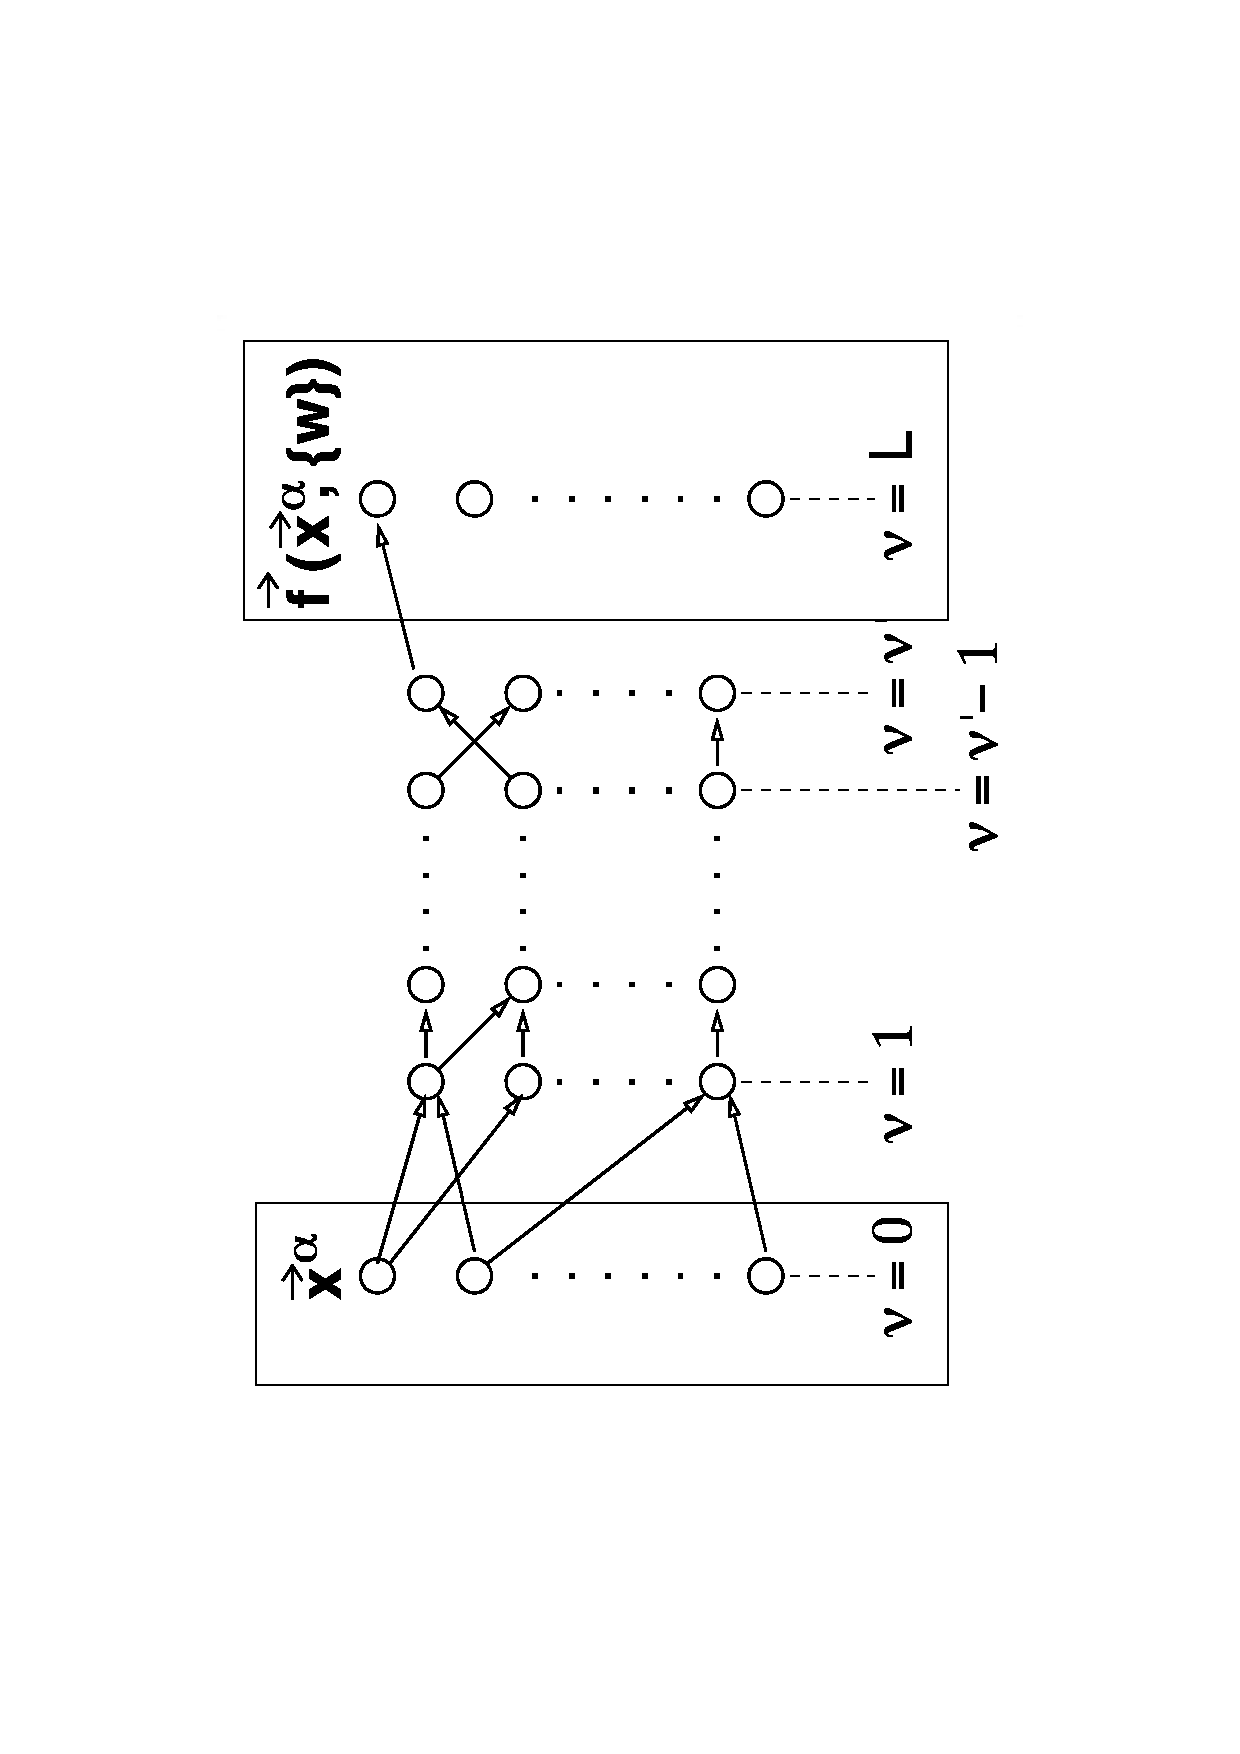
\includegraphics[angle=-90, width=.9\textwidth]{img/mlp}
		\vspace*{-40pt}
		\caption{Multilayer Perceptron (MLP)}
		\label{deployment}
	\end{figure}
	L = Anzahl der Schichten, L-1 innere Schichten (\dq hidden layers\dq)\\[5pt]
	Für jeden Knoten: %\vspace*{-10pt}
	\begin{eqnarray*}
		s_i^{v+1} &=& \sigma(\sum w_{ij}s_j^v)\\
		\sigma(a) &=& tanh(a) \text{ oder } \sigma(a) = \frac{1}{1+e^{-a}}
	\end{eqnarray*}
	\subsubsection{Modellselektion}
	\subsubsection{Kapazität}
	\begin{itemize}
		\item Jede kontinuierliche Funktion kann theoretisch mit jeglicher Genauigkeit angenähert werden
		\item Die Anzahl notwendiger Neuronen (Knoten) ist aber unbekannt
	\end{itemize}
	\subsubsection{Konkrete Modellparameter}
	\begin{itemize}
		\item Anzahl der Schichten\vspace*{-3pt}
		\begin{enumerate}[$\hookrightarrow$]
			\leftskip10pt
			\item eine innere Schicht ist ausreichend
			\item häufig funktionieren 2 Schichten aber besser
			\item modern: deep learning (viele, spezielle Schichten)
		\end{enumerate}
		\item Anzahl der Neuronen bestimmt Modellkomplexität
		\item Overfitting ist häufig ein Problem (Regularisierung notwendig)
		\item Feature extraction wichtig
	\end{itemize}
	Berechnung des Gradienten mittels Backpropagation
	\begin{itemize}
		\item Rekursive Formel zur Berechnung der Gradienten bzgl. der inneren Parameter $w_{ij}$
		\item Analytischer Ausdruck vorhanden (direkte Lösung möglich)
		\item Geringer Rechenaufwand
		\item \textbf{Backpropagation} = Methode zur Berechnung von Gradienten $\Rightarrow$ funktioniert auch für andere Modelle
	\end{itemize}
	\subsection{Lokale Modelle}
	\subsubsection{Radial Basis Funktionen-Netz (RBF)}
	\begin{figure}[ht]
		\vspace*{-60pt}
		\centering
		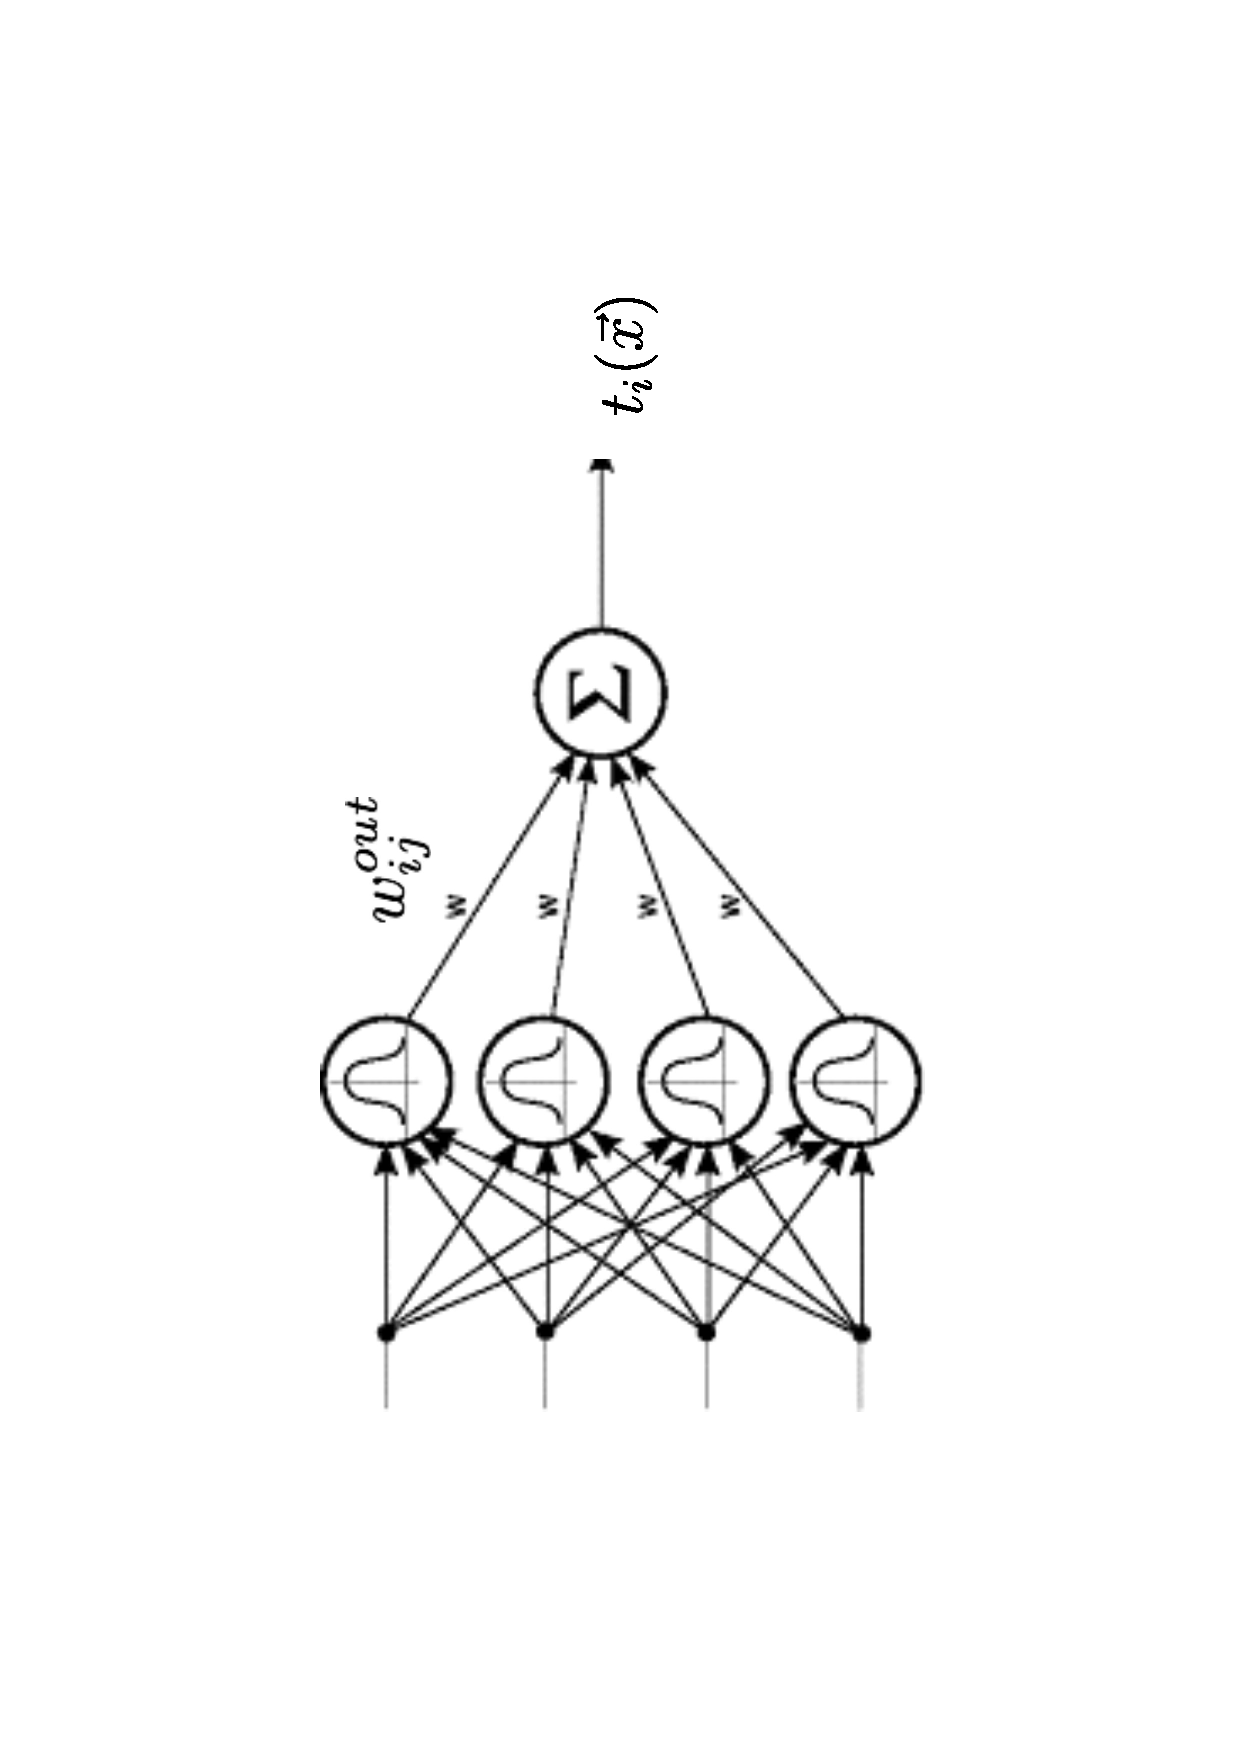
\includegraphics[angle=-90, width=.9\textwidth]{img/rbf}
		\vspace*{-60pt}
		\caption{Radiales Basis Funktionen-Netz}
		\label{deployment}
	\end{figure}
	\begin{itemize}
		\item innere Schicht aus $m=1...M$ radialen Basisfunktionen (RBF, Gaussfunktionen)
		\item lineare Kombination an der Ausgabe mit Parametern (Gewichten $w_m^{out}$)
		\begin{equation*}
		t_i(\pmb{x})=\sum_{j=1}^Jw_{ij}^{out}\cdot\Phi_j(\pmb{x}, \pmb{w_j^{in}}), \text{ mit } i \in 1,...,L ,~ j\in 1,...,J
		\end{equation*}
		\item RBF hängen nur vom Abstand des inputs zum Zentrum ab:
		\begin{equation*}
			\Phi_j(\pmb{x}, \pmb{w_j^{in}})=R(\Vert\pmb{x}-\pmb{w_j^{in}}\Vert), ~ j \in 1,...,J
		\end{equation*}\vspace*{-15pt}
		\begin{enumerate}[$\hookrightarrow$]
			\leftskip10pt
			\item $R()$ ist eine Gaussverteilung $R(s)=e^{-\frac{1}{2\sigma_j^2}s^2}$
			\item RBF: $\Phi_m(\pmb{x}, \pmb{w_j^{in}})=e^{-\frac{\Vert\pmb{x}-\pmb{w_j^{in}}\Vert}{2\sigma_j^2}}$
		\end{enumerate}
	\end{itemize}
	RBF sind:
	\begin{itemize}
		\item universelle Approximatoren
		\item lineare Modelle in der Ausgabeschicht
		\item gut verstanden, da viele Methoden um die Parameter der Gaussfunktion zu wählen
		\item die RBF-Mittelwerte können auf (einige) Daten gesetzt werden
		\item Wahl von Sigma (\dq Breite\dq) wichtig um gute Abdeckung der Daten zu erreichen
	\end{itemize}
	Berechnung:
	\begin{itemize}
		\item für L-dimensionale Ausgabe
		\begin{equation*}
			t_i(\pmb{x}) = \sum_{j=1}^M w_{ij}\cdot\Phi_j(\pmb{x}, \pmb{w_j^{in}}), ~ i\in 1,...,L, ~ j \in 1,...,M
		\end{equation*}
	\item Zusammenfassung der Parameter in Vektor $\Theta$
	\item und für 1-D Ausgabe: Linearkombination nichtlinearer RBF $\Phi$
	\begin{equation*}
		t(x) = \sum_{j=1}^M w_j\cdot\Phi_j(x, \Theta)
	\end{equation*}
	\end{itemize}
	Lösung:
	\begin{itemize}
		\item für RBF wird der quadratische Fehler des linearen Modells zu
		\begin{equation*}
			E(\pmb{w}) = \frac{1}{2}\sum_{n=1}^N(t_n-\pmb{w}^T\Phi(x_n))^2
		\end{equation*}
		\item und die Minimierung hat, wie bekannt eine analytische Lösung\vspace*{-3pt}
		\begin{enumerate}[$\hookrightarrow$]
			\leftskip10pt
			\item Ableitung bilden, gleich Null setzen, umstellen fertig!
		\end{enumerate}
		\item wie vorher
		\begin{eqnarray*}
			\pmb{\hat{w}} &=& argmin ~E(\pmb{w}) = \Vert T-\underline{\Phi}\cdot \pmb{w}\Vert\\
			&\Leftrightarrow& -\underline{\Phi}^T(T-\underline{\Phi}\cdot\pmb{w}) = 0\\
			&\Rightarrow& \pmb{\hat{w}} = (\underline{\Phi}^T\cdot\underline{\Phi})^{-1}\underline{\Phi}^T\cdot T
		\end{eqnarray*}
		\item wobei $T$ alle Daten enthält (multidimensional, dann ist $T$ Matrix)
		\item $\underline{\Phi}$ ist die Design Matrix $\Phi_{ij} = \Phi_j(\pmb{x_j})$
	\end{itemize}
	Lineare gewichtete Summe von (nichtlinearen) Gaussfunktionen ist äquivalent zu Gauss-gewichteter Summe von (konstanten) linearen Funktionen:
	\begin{equation*}
		t(x) = \sum_{j=1}^M w_j\cdot\Phi_j(x, \Theta) \Leftrightarrow t(x) = \sum_{j=1}^M \Phi_j(x, \Theta)(w_j)
	\end{equation*}
	\subsubsection{Gewichtete lineare Regression}
	Wir betrachten Regression nun mit zusätzlichen Gewichtungen für die einzelnen Datenpunkte.
	\subsubsection{Methode gewichteter kleinster Quadrate}
	\begin{equation*}
		E(\pmb{w})=\frac{1}{2}\sum_{n=1}^Nd_n(t_n-\pmb{a}^Tx_n)^2
	\end{equation*}
	mit $\pmb{a}$ als Parametervektor für eine Gerade\\[5pt]
	Hinweis: Im einfachen linearen Modell werden hier die Datenpunkte direkt verwendet und nicht vorverarbeitet $\Phi_m(\pmb{x})=x_m$.\\
	Die Lösung der Normalengleichung wird dann zu
	\begin{equation*}
		\pmb{a^*} = (\Phi^TD\Phi)^{-1}\Phi^TD\pmb{t} = (X^TDX)^{-1}X^TD\pmb{t}
	\end{equation*}
	mit $D_{nn} = d_n$, wobei $D$ eine diagonale Skalierungs-Matrix darstellt $D=\begin{pmatrix}
			d_1 & ... &  \\
	\vdots & \ddots & \vdots \\
	 & ... & d_n)
	\end{pmatrix}$.\\
	Als Gewichtsfunktion wird die Dichtefunktion der Normalverteilung mit Mittelwert $\mu_1$ und Kovarianz $\Sigma$ genutzt:
	\begin{equation*}
		d_n=\Phi(x_n, \Theta) = N(x_n\vert\mu_1,\Sigma) = e^{-\frac{1}{2}(x-\mu_1)^T\Sigma^{-1}(x-\mu_1)}
	\end{equation*}
	damit tragen nur Datenpunkte in der Nähe des Erwartungswertes effektiv zum Fehler bei.
	\subsubsection{Lokale gewichtete Regression (LWR)}
	\begin{itemize}
		\item bestimme mehrere Geraden-Segmente für verschiedene Gauß-Kurven, die jeweils mit $\mu_e, \Sigma_e$ parametrisiert sind
		\begin{equation*}
			\pmb{a_e} = (X^TD_eX)^{-1}X^TD_e\pmb{t}, \text{ für } e=1...E
		\end{equation*}
		mit Gaussverteilter Gewichtsfunktion mit $\Theta = (\mu_e;\Sigma_e)$
		\item finale Modell wird dann als Summe überlagerter, linear skalierter Gauß-Funktionen bzw. aus überlagerten Geradensegmenten gebildet:
		\begin{equation*}
			t(x) = \sum_{e=1}^E\Phi(x, \Theta_e)(\pmb{a_e}^Tx)
		\end{equation*}
		\item es ist auch möglich die Geraden zu verschieben
		\begin{equation*}
			t(x) = \sum_{e=1}^E\Phi(x, \Theta_e)(\pmb{a_e}^Tx+ b_e)
		\end{equation*}
	indem eine erweiterte Regressions-Matrix verwendet wird\\ X=$\begin{pmatrix}
	x_{11} & ... & x_{1p} & 1\\
	\vdots & \ddots & \vdots & 1\\
	x_{n1} & ... & x_{np} & 1
	\end{pmatrix}, x_n \in R^p$\\[5pt]
	Hinweis: hier ist $X$ die (erweiterte) Designmatrix für die \dq innere Regression\dq, da ja $\Phi_m(\pmb{x})=x_m$.
	\end{itemize}
	RBF ist Spezialfall von LWR ($E=M, b_e=w_e, a \equiv 0$).\vspace*{-5pt}
	\begin{enumerate}[$\hookrightarrow$]
		\leftskip10pt
		\item Das RBF kann als Summe sehr einfacher Modelle (einer Konstanten $w_j$) verstanden werden, die mit Gauss-Funktionen gewichtet sind.
	\end{enumerate}
	Damit:\\[5pt]
	LWR: Überlagerung von Geraden, die lokal gewichtet sind.\vspace*{-5pt}
	\begin{enumerate}[$\hookrightarrow$]
		\leftskip10pt
		\item benötigt $E$ Regressionsschritte und ist nichtlinear in den Parametern
		\item ist ein allgemeineres Modell
	\end{enumerate}
	RBF: Überlagerung von konstanten Funktionen mit Gaußgewichten.\vspace*{-5pt}
	\begin{enumerate}[$\hookrightarrow$]
		\leftskip10pt
		\item benötigt nur einen Schritt, da linear in den Parametern
	\end{enumerate}
	\subsubsection{Vereinheitlichtes Modell (unified modell)}
	Viele Algorithmen verwenden die gleiche Modellform. Daher kann die gegebene Form
	\begin{equation*}
		t(x) = \sum_{e=1}^E\Phi(x, \Theta_e)(\pmb{a_e}^Tx+ b_e)
	\end{equation*}
	als vereinheitlichtes (unified) Modell verstanden werden.\\[5pt]
	Spezialfälle sind zum Beispiel:
	\begin{itemize}
		\item einfache lineare Regression
		\item RBF
		\item Gauß-gewichtete lineare Regression
		\item Gauß-gewichtete lokale lineare Regression
		\item auch probabilistische Modelle
		\item noch weitere Modelle
	\end{itemize}
	\subsection{Modellierung von Unsicherheit (statistischer Ansatz)}
	Annahmen:
	\begin{itemize}
		\item $\pmb{w^*}$ ist echter Parameter eines parametrisierten Modells
		\item Daten sind verrauscht $t_n=f(x_n,\pmb{w})+\nu$
		\item durch einen der besprochenen Algorithmen (z.B. Maximum Likelihood) erhalten wir eine Schätzung für den echten Parameter $\pmb{w^*}$:
		\begin{equation*}
			\pmb{\hat{w}}(Z),~Z=(X,T)
		\end{equation*}\vspace*{-20pt}
		\begin{enumerate}[$\hookrightarrow$]
			\leftskip10pt
			\item $\pmb{\hat{w}}(Z)$ wird \textbf{Schätzer} genannt und ist selbst eine Zufallsvariable, weil die Daten $Z$ verrauscht sind.
			\item Versuch mit neuen Daten wiederholen um einen neuen Schätzer zu berechnen $\pmb{\hat{w}'}(Z)$
		\end{enumerate}
	\end{itemize}
	Gewünschte Eigenschaften:
	\begin{itemize}
		\item ein Schätzer sollte \textbf{erwartungstreu} (unbiased) sein:
		\begin{itemize}
			\item liefert im Mittel den \dq wahren\dq Parameter
			\item d.h. der Schätzer macht keinen systematischen Fehler
			\item Erinnerung: braucht die Annahme, dass es einen \dq wahren\dq Parameter $\pmb{w^*}$ gibt
			\item falls es einen Bias (= systematische Abweichung) gibt, kann man diesen manchmal ausrechnen und diesen dann wiederum in den Schätzer integrieren
		\end{itemize}
		\item ein Schätzer sollte minimale Varianz haben
		\begin{itemize}
			\item geringe Varianz erhöht die Wahrscheinlichkeit bei einer/wenigen Durchführungen des Experimentes dem wahren Wert nahe zu kommen
		\end{itemize}
	\end{itemize}
	\textbf{Aber:} Es gibt nicht immer einen erwartungstreuen Schätzer.\\[5pt]
	$\Rightarrow$ Schätzer soll erwartungstreu und eine minimale Varianz besitzen\\\hspace*{10pt} $<(\pmb{\hat{w}}-<\pmb{\hat{w}}>)^2> ~\rightarrow ~min$.\vspace*{-5pt}
	\begin{enumerate}[$\hookrightarrow$]
		\leftskip10pt
		\item diese Schätzer werden als \textbf{UMV} (unbiased minimal variance) bezeichnet
	\end{enumerate}
	\subsubsection{Cramer-Rao Grenze}
	Es gibt eine untere Grenze für die Varianz von erwartungstreuen Schätzern, die mit der log-likelihood $l(\pmb{w})$ verbunden ist:
	\begin{equation*}
		Var(\pmb{\hat{w}}) \ge \frac{1}{-<\frac{\delta^2l(\pmb{w})}{\delta\pmb{w}^2}>} =\frac{1}{<(\frac{\delta l}{\delta w})^2>}
	\end{equation*}
	Interpretation: Je flacher (gemessen durch die mittlere Krümmung, bzw. Ableitung) die log-likelihood Funktion, desto größer die minimal erreichbare Varianz.\\
	$\Rightarrow$ Schätzer, die diese Grenze erreichen werden \textbf{effizient} genannt.
	\begin{equation*}
		-<\frac{\delta^2l(\pmb{w})}{\delta\pmb{w}^2}>_{\pmb{z}} \begin{cases}
		\text{large}\\
		\text{small}
		\end{cases} \Leftrightarrow Var(\pmb{\hat{w}}) \begin{cases}
		\text{small}\\
		\text{large}
		\end{cases}
	\end{equation*}
	Bestimmung von effizienten Schätzern:
	\begin{itemize}
		\item Die Cramer-Rao Grenze ist erreicht, wenn folgendes gilt
		\begin{equation*}
			Var(\pmb{\hat{w}}) <(\frac{\delta l}{\delta w})^2> = 1
		\end{equation*}
		\item Es gibt eine Zerlegung der folgenden Form
		\begin{equation*}
			\frac{\delta lnP(\pmb{z}\vert \pmb{w})}{\delta \pmb{w}} = \lambda(\pmb{w}) \cdot (\pmb{\hat{w}}(\pmb{z})-\pmb{w})
		\end{equation*}
		Mit den Funktionen $\lambda(\pmb{w}), \pmb{\hat{w}}(\pmb{z})$ und dem wahren Parameter $\pmb{w}$
		\item $\lambda(\pmb{w}) = Var(\pmb{\hat{w}}(\pmb{z}))^{-1}$ und $\pmb{\hat{w}}(\pmb{z})$ sind effiziente Schätzer
	\end{itemize}
	\subsubsection{Lineare Regression zur Schätzung}
	Betrachte das generelle, lineare, stochastische Modell mit nichtlinearer Eingangsfunktion $\Phi(\pmb{x})$
	\begin{equation*}
		y = w_0 + \sum_{j=1}^M w_j\Phi_j(\pmb{x}) + \nu
	\end{equation*}
	Wir definieren $\pmb{x}$ als Datenvektor nach der Vorverarbeitung neu $\pmb{x}_k = (\Phi_1(x_k),..., \Phi_M(x_k))^T \in \mathbb{R}^M$. Mit der folgenden Notation lässt sich das Modell sehr kompakt schreiben:
	\begin{eqnarray*}
		X &=& \begin{pmatrix}
				1 & 1 & ... & 1\\
				\pmb{x}_1 & \pmb{x}_2 & ... & \pmb{x}_k
		\end{pmatrix}^T \in \mathbb{R}^k \times \mathbb{R}^{M+1}\\
		\pmb{w} &=& (w_0,...,w_k)^T \in \mathbb{R}^k\\
		\pmb{\nu} &=& (\nu_1,...,\nu_k)^T \in \mathbb{R}^k\\
		\pmb{y} &=& (y_1,...,y_k)^T \in \mathbb{R}^k\\
		\pmb{y} &=& X\pmb{w}+\pmb{\nu}
	\end{eqnarray*}
	Dafür erhalten wir mit der Zerlegung die folgenden Schätzer
	\begin{eqnarray*}
		\Lambda(\pmb{w}) &=& \frac{1}{\sigma^2}X^TX\\
		\pmb{w}(z) &=& (X^TX)^{-1}X^T\pmb{y}\\
		\Rightarrow \pmb{\hat{w}} &=& (X^TX)^{-1}X^T\pmb{y}
	\end{eqnarray*}
	\subsubsection{Maximum Likelihood als Schätzer}
		\begin{figure}[ht]
		\centering
		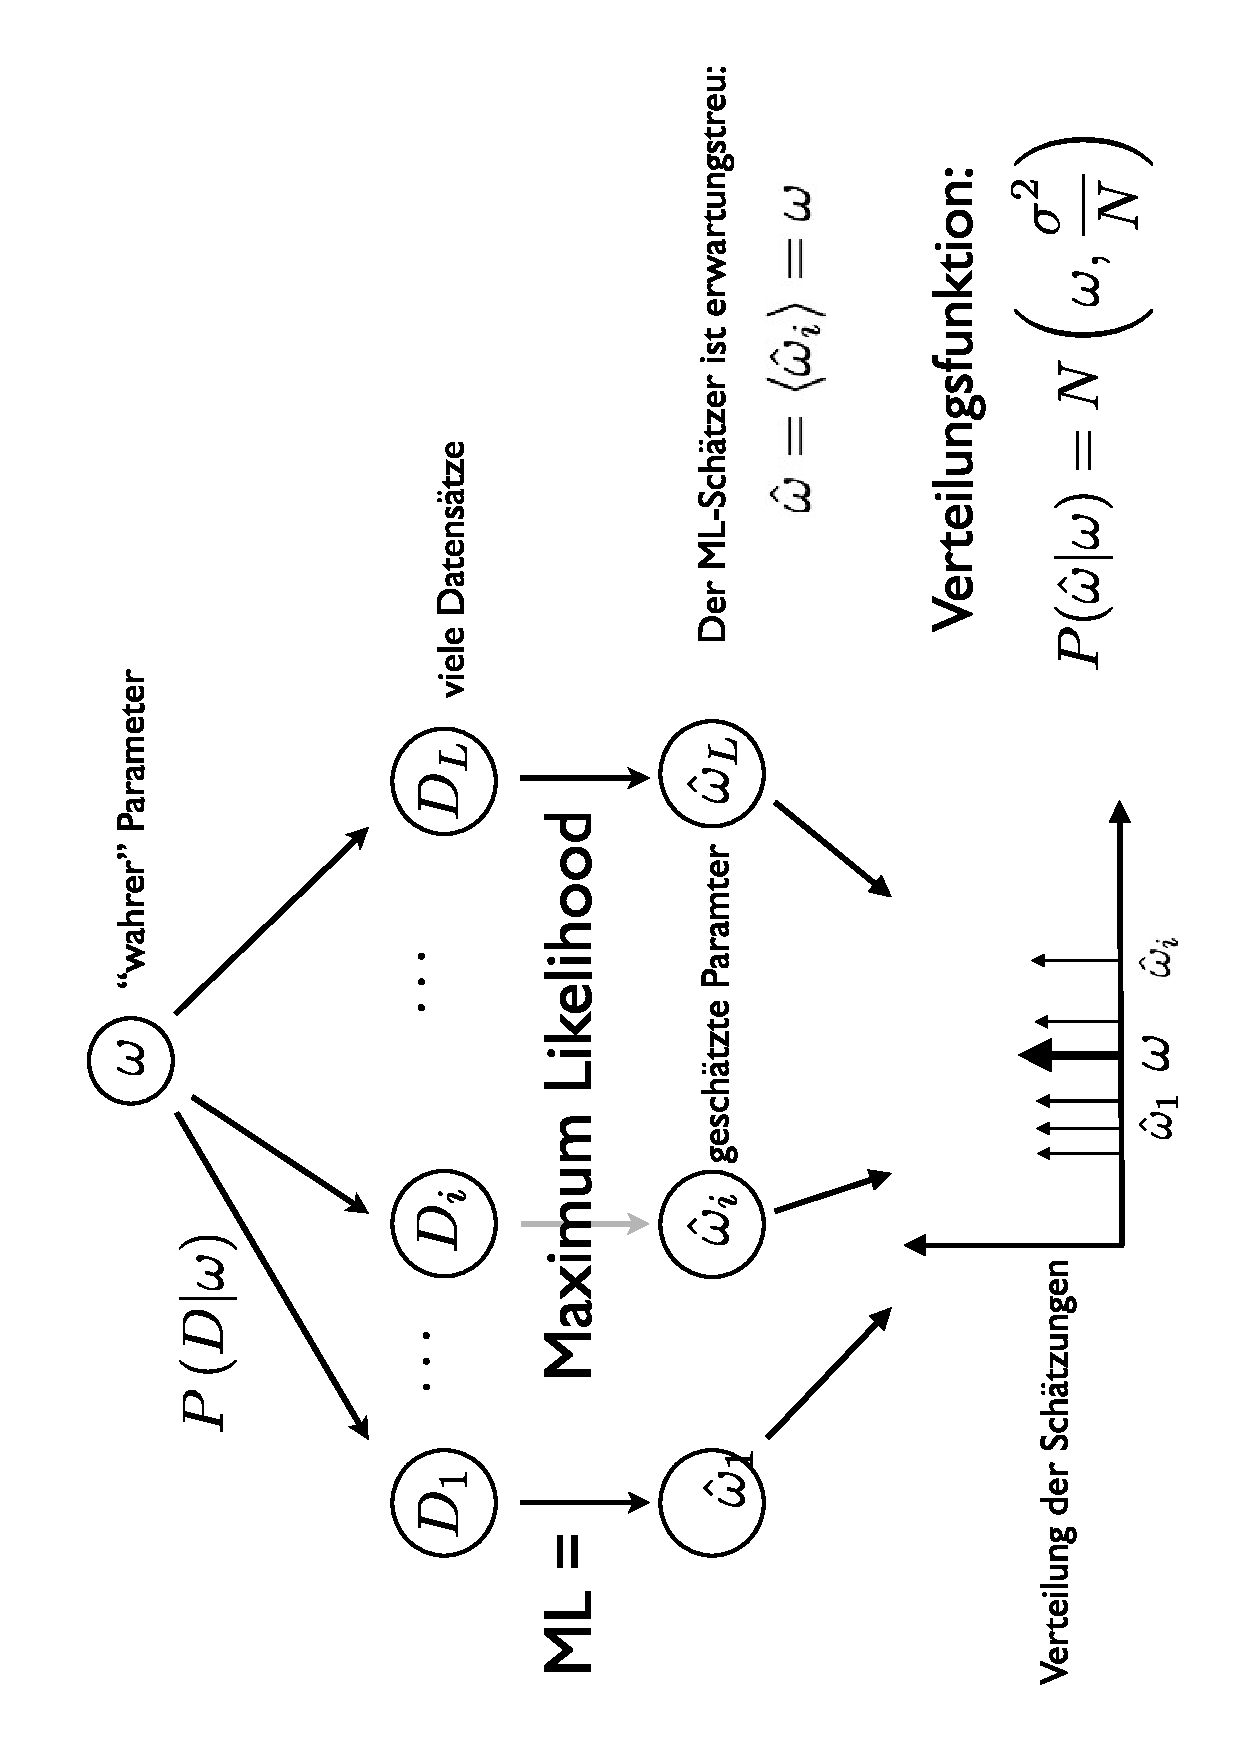
\includegraphics[angle=-90, width=.9\textwidth]{img/ml_schaetzer}
		\caption{Die statistische Interpretation des Likelihood}
		\label{deployment}
	\end{figure}
	In der Theorie liefert die Maximum Likelihood Methode UMV Schätzer, wenn ein Parameter gefunden werden kann, der die Likelihood maximiert
	\begin{eqnarray*}
		\pmb{\hat{w}}(D) &=&~argmax~P(D\vert \pmb{w})\\
		P(\pmb{\hat{w}}\vert \pmb{w}) &\sim& N(\pmb{w}\vert \frac{\sigma^2}{N}) 
	\end{eqnarray*}
	\begin{itemize}
		\item der Schätzer ist dann selbst normalverteilt um den Mittelwert
		\item die Varianz nimmt mit zunehmender Datenmenge ab
	\end{itemize}
	In der Praxis wissen wir, dass wir den Fehler minimieren müssen aber häufig nur lokale Minima finden können.
	\subsection{Klassifikation}
	Aufgabe: Ordne Datum $x$ einer von $K$ diskreten, disjunkten Klassen zu.\vspace*{-5pt}
	\begin{enumerate}[$\hookrightarrow$]
		\leftskip10pt
		\item sofern die Klassen linear trennbar sind, können die Grenzen durch Hyperebenen dargestellt werden
	\end{enumerate}
	\subsubsection{Linear separierbarer Fall}
	Definition einer Hyperebene:
	\begin{equation*}
		\pmb{w}^T\pmb{x} +w_0 = 0 ~(\text{Gerade für } \pmb{x} \in \mathbb{R}^2)
	\end{equation*}
	Zuordnung (hier für zwei Klassen):\\[5pt]
	Klasse 0 : $\pmb{w}^T\pmb{x} +w_0 < 0$,\\
	Klasse 1: $\pmb{w}^T\pmb{x} +w_0 > 0$, \\
	Grenze : $\pmb{w}^T\pmb{x} +w_0 = 0$.\\[5pt]
	$K = 2$ Klassen:\\[5pt]
	Hier gilt für die Label/Sollausgaben $t$:
	\begin{equation*}
		t \in \{-1, 1\} \text{ oder } t \in \{0, 1\}
	\end{equation*}\vspace*{-5pt}
	\begin{enumerate}[$\hookrightarrow$]
		\leftskip10pt
		\item Die Label können im letzteren Fall als Wahrscheinlichkeit interpretiert werden
	\end{enumerate}
	$K > 2$  Klassen:\\[5pt]
	Hier wird gewöhnlich die 1-of-$K$ Kodierung verwendet
	\begin{eqnarray*}
		\pmb{t} &=& (0,...,0,1,0,...,0) \in \mathbb{R}^K\\
		t_k &=& 1 \Leftrightarrow x \in C_k
	\end{eqnarray*}
	wobei $C_k$ die $k$-te Klasse bezeichnet.\\[5pt]
	Drei Ansätze:
	\begin{enumerate}
		\item Finde eine direkte Abbildung $f$ von den Eingängen auf die Klassen.
		\begin{itemize}
			\item $f$ heißt Diskriminatenfunktion (\textbf{Diskriminate})
			\item Wahrscheinlichkeiten werden nicht betrachtet
			\begin{equation*}
				f(x): x \rightarrow 0,1
			\end{equation*}
		\end{itemize}
		\item Bayes'scher Ansatz:
		\begin{enumerate}
			\item Modellieren der Likelihood
			\item Modellierung der a-priori Wahrscheinlichkeiten für jede Klasse
			\item Berechne im nächsten Schritt den Posterior $p(C_k\vert x)$
		\end{enumerate}
		\item Direkte Modellierung des Posteriors
	\end{enumerate}
	\subsubsection{Fisher-Diskriminante}
	Ansatz zur linearen Trennung (d.h. Diskriminante $f$ ist Hyperebene)
	\begin{itemize}
		\item berechne Projektion der Daten auf eine Linie
		\item optimiere die Wahl der Linie um beste Trennung zu erreichen
		\item wähle Wert auf der Linie, zur Diskriminierung
	\end{itemize}
	Berechnung (zwei Klassen $C_1, C_2$ mit $N_1, N_2$ Punkten):
	\begin{itemize}
		\item Mittelwert $m_{1/2}$
		\item Projektion von 2D auf 1D mit linearem Modell
		\begin{equation*}
			y(\pmb{x} = \pmb{w}^T\pmb{x})
		\end{equation*}\vspace*{-5pt}
		\begin{enumerate}[$\hookrightarrow$]
			\leftskip10pt
			\item Projizierte Punkte liegen auf Geraden in Richtung $\pmb{w}$
			\item Projektion verläuft senkrecht
		\end{enumerate}
		\item einfacher Ansatz: Abstand der projizierten Mittelwerte maximieren (maximize inter-class variance)
		\begin{equation*}
			max~ \vert m_1'-m_2'\vert \Leftrightarrow~max~\vert\pmb{w}^T\cdot m_1 - \pmb{w}^T\cdot m_2\vert
		\end{equation*}
		$\Rightarrow \pmb{w}\propto (m_2-m_1)$ ($\pmb{w}$ zeigt in Richtung $m_2-m_1$)
		Beachte: 
		\begin{itemize}
			\item Richtung, Länge von $\pmb{w}$ unwichtig
			\item Projektionen können stark überlappen
		\end{itemize}
		\item Besser: Zusätzlich die Varianz innerhalb der Klasse minimieren (minimize intra-class varianz)
		\begin{equation*}
			s_k^2=\sum_{x_n \in C_k} (w_nx_n-m_k')^2
		\end{equation*}
		Dann maximiere die folgende Kostenfunktion:
		\begin{equation*}
			J(\pmb{w}) = \frac{(m_1'-m_2')^2}{s_1^2+s_2^2}
		\end{equation*}
		\item $J(\pmb{w})$ wird maximal, wenn gilt:
		\begin{eqnarray*}
			\pmb{w} &\propto& S_{\pmb{w}}^{-1}(m_2-m_1)\\
			S_{\pmb{w}} &=& \sum_{x_n \in C_1} (x_n-m_1)(x_n-m_1)^T + \sum_{x_n \in C_2}(x_n-m_2)(x_n-m_2^T)
		\end{eqnarray*}
	\end{itemize}
	Bemerkung: Abstand zwischen Mittelwerten nicht mehr maximal. Es lässt sich zeigen, dass das selbe Ergebnis durch Minimierung des quadratischen Fehlers erzielt werden kann
	\begin{equation*}
		E(\pmb{w}) = \frac{1}{2}\sum_{n=1}^N(\pmb{w}^Tx_n +w_0 -t_n)^2 \text{ mit } t_n = \frac{N}{N_n}
	\end{equation*}
	Achtung: die traditionelle Bezeichnung \dq Fisher Diskriminante\dq ist etwas irreführend!
	\begin{itemize}
		\item Vektor $\pmb{w}$ gibt nur Projektionsgerade an, nicht die Klassengrenze
		\item Diskriminierungsfunktion notwendig
	\end{itemize}
	Optimale Klassifikation für neuen Datenpunkt $x \in C_1$ wenn $\pmb{w}^T(x-m)>0$ und sonst in der anderen Klasse.
	\subsubsection{Bayes'scher Ansatz}
	\begin{itemize}
		\item modelliere die Likelihood $p(x\vert C_k)$ und Prior $p(C_k)$ (hier Likelihood = class conditional)\vspace*{-3pt}
		\begin{enumerate}[$\hookrightarrow$]
			\leftskip10pt
			\item Indirekter Ansatz um die Wahrscheinlichkeit für eine Klasse (posterior) $p(C_k\vert x)$ zu finden
		\end{enumerate}
		\item Bayes Theorem für 2 Klassen:
		\begin{equation*}
			p(C_1\vert x) = \frac{p(x\vert C_1)p(C_1)}{p(x\vert C_1)p(C_1)+p(x\vert C_2)p(C_2)} = \frac{1}{1+e^{-a}}, ~a = ln\frac{p(x\vert C_1)p(C_1)}{p(x\vert C_2)p(C_2)}
		\end{equation*}
		\item Generalisierung für $k>2$ Klassen:
		\begin{equation*}
			p(C_k\vert x) = \frac{p(x\vert C_k)p(C_k)}{\sum_j p(x\vert C_j)p(C_j)} = \frac{exp(a_k)}{\sum_j exp(a_j)} \text{ (softmax Funktion)}, ~a_j = ln~p(x\vert C_j)p(C_j)
		\end{equation*}
		\item die Softmax Funktion kann als kontinuierliche differenzierbare Version des Maximums verstanden werden. Wenn $a_k >>a_j$ dann gilt: $p(C_K\vert x)\approx 1, p(C_j\vert x)\approx 0, j\ne k$
	\end{itemize}
	Der Bayes'sche Ansatz mit sigmoiden Funktionen führt zu einer einfachen Lösung wenn die Klassen als Normalverteilungen modelliert werden.
	\begin{itemize}
		\item Annahme: gleiche Kovarianz
		\begin{equation*}
			p(x\vert C_k) = \frac{1}{2\pi^{\frac{D}{2}}}\frac{1}{\vert\Sigma\vert^\frac{1}{2}}exp(-\frac{1}{2}(x-\mu_k)^T\Sigma^{-1}(x-\mu_k)
		\end{equation*}
		\item für den Posterior erhält man dann lineare Klassengrenzen:
		\begin{equation*}
			p(C_1\vert x) = \sigma(ln\frac{p(x\vert C_1)p(C_1)}{p(x\vert C_2)p(C_2)})
		\end{equation*}
		\item dies wird auch \textbf{generalized linear model} genannt, wobei die Ausgabe durch die sigmoid Funktion nichtlinear wird und als Wahrscheinlichkeit interpretierbar ist
		\begin{eqnarray*}
			p(C_1\vert x) &=& \sigma(\pmb{w}^Tx+w_0)\\
			\pmb{w} &=&\Sigma^{-1}(\mu_1-\mu_2)\\
			w_0 &=& -\frac{1}{2}\mu_1\Sigma^{-1}\mu_1+\frac{1}{2}\mu_2\Sigma^{-1}\mu_2+ln\frac{p(C_1)}{p(C_2)}
		\end{eqnarray*}
		Anmerkung: Wegen der Annahme gleiche Kovarianz kürzen sich bei der Berechnung die Normalisierungsterme und quadratischen $x$-Terme heraus
	\end{itemize}
	Direkter Maximum Likelihood für Labels:
	\begin{itemize}
		\item direkter Ansatz um Daten auf Labels abzubilden
		\item Voraussetzung: gelabelte Daten $(x_n,t_n)$
		\item Annahmen:
		\begin{itemize}
			\item wie vorher: $p(x\vert C_k)$ normalverteilt
			\item Prior gegeben als $\pi = p(C_1) = 1-p(C_2)$
		\end{itemize}
		\item Damit wird Label-Data-Likelihood zu
		\begin{equation*}
			p(\pmb{t}\vert \pi, \mu_1, \mu_2, \Sigma) =L(\pi, \mu_1, \mu_2, \Sigma) = \prod_n [\pi N(\pmb{x}\vert \mu_1, \Sigma)]^{t_n}[(1-\pi)N(\pmb{x}\vert \mu_2,\Sigma)]^{1-t_n}
		\end{equation*}
		\item argmax log L() liefert optimale Parameter
		\item Likelihood zur Zuordnung von Labels auf neue Daten
	\end{itemize}
	Berechnung:
	\begin{itemize}
		\item zuerst nur für Terme die von $\pi$ abhängen
		\begin{equation*}
			argmax_\pi ~ \sum_n(t_nln(\pi)+(1-t_n)ln(1-\pi))
		\end{equation*}
		\begin{equation*}
			\Rightarrow \pi = \frac{1}{N}\sum_n t_n = \frac{N_1}{N} \Leftrightarrow 1-\pi = \frac{N_2}{N}
		\end{equation*}
		\item intuitiv richtig: A-priori $\sim$ Anzahl der Punkte in der jeweiligen Klasse
		\item Mittelwert und Kovarianz
		\begin{eqnarray*}
			\mu_1 &=& \frac{1}{N_1}\sum_{n=1}^Nt_nx_n\\
			\mu_2 &=& \frac{1}{N_2}\sum_{n=1}^N(1-t_n)x_n\\
			\Sigma &=& \frac{N_1}{N}s_1+\frac{N_2}{N}s_2\\
			s_i &=& \frac{1}{N_i}\sum_{x_n \in C_i}(x-\mu_i)(x-\mu_i)^T
		\end{eqnarray*}
		\item intuitiv richtig: Summe der Intra-Klassen-Varianzen
	\end{itemize}
	\subsubsection{Probabilistische Diskriminierung}
	\begin{itemize}
		\item Posterior als Funktion von $x$ modellieren
		\begin{equation*}
			p(C_k\vert x) = y(x_n) = \sigma(\pmb{w}^Tx_n), x_n \in C_k
		\end{equation*}
		\item diese Modelltypen nennen sich \textbf{logistische Regression}
		\item andere Herangehensweise: Vorgabe des Modells in Sigmoid Funktion
		\item optimiere Parameter der log-Likelihood
		\begin{equation*}
			p(\pmb{t} \vert \pmb{w}) = \prod_n y_n^{t_n}(1-y_n)^{(1-t_n)}
		\end{equation*}
		\begin{equation*}
			argamx_{\pmb{w}}~-log~L(\pmb{w})
		\end{equation*}
		\begin{equation*}
			 = -\sum_{n=1}^N ln(y_n^{t_n})+ ln((1-y_n)^{(1-t_n)})
		\end{equation*}
		\item Dies entspricht der Minimierung der sogenannten \textbf{cross-entropy}
		\begin{equation*}
			E(\pmb{w}) = -\sum_{n=1}^N \underbrace{t_nln(y_n)}_\text{0 für $t_n = 0$}+ \underbrace{(1-t_n)ln(1-y_n)}_\text{0 für $t_n=1$}
		\end{equation*}
		\item $y(x)$ ist dann direkt als Wahrscheinlichkeit $p(C_1\vert x)$ (posterior) zu interpretieren
		\item Optimierung mittels \textbf{gradient descent}\vspace*{-3pt}
		\begin{enumerate}[$\hookrightarrow$]
			\leftskip10pt
			\item Analytische Lösung
			\item Erweiterung auf mehrere Klassen
		\end{enumerate}
	\end{itemize}
\newpage
	\subsection{Konzeptlernen}
	\begin{itemize}
		\item behandelt den allgemeinen Fall nicht numerischer Daten
		\item Abstraktes Framework zur Betrachtung von Mengen/Teilmengen
		\item $X$ := Menge von Instanzen $x$
		\item $C$ := \textbf{Konzept} = Untermenge von $X$ = Funktion $c:X\rightarrow\{0,1\}$ (\textbf{Indikator}) beschreibt Untermenge
		\item Anzahl der möglichen Konzepte $2^{\vert X\vert}$
		\item Beschreibung des Konzepts = Klassifikation aller Elemente von $X$ 
	\end{itemize}
	Konzeptlernen: Gewinnung einer boolschen Funktion aus den Instanzen und deren Label in den Trainingsdaten.\\[5pt]
	Äquivalent: Identifizierung einer bestimmten Untermenge aus den Trainingsdaten.
	\subsubsection{Hypothesenraum}
	\begin{itemize}
		\item suche im gesamten Konzeptraum zu komplex
		\item schränke die Suche auf weniger Funktionen/Teilmengen ein
		\item $H$ := Hypothesenraum von Funktionen $h$
		\begin{equation*}
			h:X\rightarrow\{0,1\}
		\end{equation*}
		\item äquivalent: reduziere Anzahl möglicher Untermengen
		\item Hypothesenraum drückt Annahme über das Problem aus (Bias)
		\begin{itemize}
			\item ermöglicht Generalisierung
			\item induktives Hypothesenlernen
		\end{itemize}
		\item Grundannahme (\textbf{inductive learning bias}): Jede Hypothese, die die Zielfunktion auf einem genügend großen Datensatz annähert ist auch eine gute Hypothese für den gesamten Raum $X$
	\end{itemize}
	Spezialfall: Beschreibung durch Attribute
	\begin{itemize}
		\item Datenbeschreibung als Tupel diskret-wertiger Attribute\\ 
		(\dq Wert(Attribut 1)\dq, \dq Wert(Attribut 2)\dq, ...)\\
		N = \#Kombinationen = \#Wert(Attribut 1) $\cdot$ \#Wert(Attribut 2)$\cdot$... $\rightarrow 2^N$ Konzepte
	\end{itemize}
	\subsubsection{Hypothesen}
	\begin{itemize}
		\item Konjunktionen von Bedingungen an die Attribute
		\item \dq constraint(Attribut 1)\dq $\land$ \dq constraint(Attribut 2)\dq $\land$ ...
		\item mögliche constraints:
		\begin{itemize}
			\item $?$ = alle Werte sind erlaubt
			\item $\emptyset$ = kein Wert ist erlaubt
			\item $v$ = nur der Wert $v$ ist erlaubt
		\end{itemize}
	\end{itemize}
	\textbf{Bemerkung:} Es gibt Hypothesen die semantisch äquivalent aber syntaktisch verschieden sind. Es gibt mehr Konzepte als semantisch verschiedene Hypothesen.\\[5pt]
	Allgemeinere oder genauso allgemeine (\textbf{generelle}) Hypothesen:
	\begin{equation*}
		h_i \ge_g h_j
	\end{equation*}
	$h_i$ ist genereller als $h_j$ genau dann wenn $\forall x \in X: (h_j(x)=1 \Rightarrow h_i(x)=1$.\\[5pt]
	Strikt mehr generelle Hypothesen:\\[5pt]
	\dq ist genereller als\dq = \dq schließt die gleiche oder Obermenge ein\dq\\ $h_i \ge_g h_j$\\ $(h_i \ge_g h_j) \land (h_i \ne h_j)$\\ $\{x \in D \vert h_i(x) = 1\} \subseteq \{x\in D\vert h_j(x)=1\}$\\[5pt]
	Einfachster Algorithmus für attributbezogene Daten:	
	\begin{algorithm}
		\caption{Generalisierung (nur positive Daten)}\label{euclid}
		\begin{algorithmic}[1]
			\State INIT $h$ with $<\emptyset, \emptyset, ...>$ \Comment{Initialisierung mit spezifischer Hypothese}
			\ForAll {positive examples $x$} \Comment{Iteriere über alle Trainingsdaten}
				\ForAll {constraints $a_i$}\Comment{Iteriere über alle attribute Bedingungen}
					\If {$a_i$ is fullfilled by $x$} \Comment{Wenn Bedingung für Datenpunkt erfüllt ist}
						\State{OK}
					\Else
						\State{generalize $a_i$} \Comment{Ansonsten wähle generellere Bedingung. Ersetze die Bedingung $a_i$ mit der nächst generelleren Bedingung $a_j$, für die $x$ die Bedingung erfüllt}
					\EndIf
				\EndFor
			\EndFor
		\end{algorithmic}
	\end{algorithm}\\
	\textbf{Probleme:}
	\begin{itemize}
		\item nur positive Beispiele werden verwendet
		\item Konvergenz kann nicht geprüft werden
		\item nicht robust gegen fehlerhafte Daten
	\end{itemize}
	\subsubsection{Versionsraum}
	Eine Hypothese ist \textbf{konsistent} auf Beispielmenge $D$ $\Leftrightarrow h(x) = c(x), \forall x \in D$. Das heißt die Hypothese klassifiziert korrekt für alle Datenpunkte in $D$. Die Menge aller konsistenten Hypothesen heißt \textbf{Versionsraum} $V_{H,D}$.\\[5pt]
	Der Versionsraum lässt sich durch zwei Hypothesensätze vollständig beschreiben:
	\begin{eqnarray*}
		G &:=& \set{g\in H\vert g \text{ ist konsistent und } \lnot \exists g': g' >_g g \land g' \text{ konsistent}}\\
		G &=& \text{Satz generellster konsistenter Hypothesen}\\
		S &:=& \set{s\in H\vert s \text{ ist konsistent und } \lnot \exists s': s>_g s' \land s' \text{ konsistent}}\\
		S &=& \text{Satz spezifischster konsistenter Hypothesen}
	\end{eqnarray*}
	Damit wird der Versionsraum durch $G$ und $S$ begrenzt definiert:
	\begin{equation*}
		V_{H,D} = \set{h\in H\vert (\exists s \in S)(\exists g \in G): g \ge_g h\ge_g s}
	\end{equation*}
	\subsubsection{Kandidateneliminierung}
	Eliminiere Hypothesen um Versionsraum zu erhalten. Kombiniere dazu die Ansätze Generalisierung und Spezialisierung.
	\begin{algorithm}
		\caption{Kandidateneliminierung}\label{euclid}
		\begin{flushleft}
			\textbf{OUTPUT:} Versionsraum
		\end{flushleft}
		\begin{algorithmic}[1]
			\ForAll {examples $x$}
				\If {example positive}
					\State{generalize $S$}
				\ElsIf {example negative}
					\State{specialize $G$}
				\EndIf
			\EndFor
		\end{algorithmic}
	\end{algorithm}\\
	Konvergiert zu eine richtigen Konzept $C$, wenn $h=c \in H$ und alle Beispiele richtig klassifiziert werden.\\[5pt]
	\textbf{Problem:} Wenn ein Datenpunkt falsch gelabelt (inkonsistent) ist, wird die korrekte Hypothese fälschlicherweise gelöscht.
	\begin{itemize}
		\item Falls Versionsraum nur eine Hypothese enthält, verwende diese
		\item Falls Versionsraum noch viele Hypothesen zulässt
		\begin{itemize}
			\item Generell mögliche Klassifikationsregel: Mehrheit + Konfidenz
		\end{itemize}
	\end{itemize}
	\subsubsection{Induktiver Bias}
	\begin{itemize}
		\item $L$ sei ein Konzeptlerner (Algorithmus)
		\item Für $X$ gelte:
		\begin{eqnarray*}
			c &=& \text{Konzept}: c:X\rightarrow \set{0,1}\\
			D &=& \set{x, c(x)} = \text{Trainingsdatensatz (korrekt gelabelt)}
		\end{eqnarray*}
	\item Bezeichne mit $L(x),c$ die Klassifizierung von $x\in X$ nach Training $D$
	\item Dann heißt ein willkürlicher Satz von Annahmen $B$ induktiver Bias von $L$ wenn für $c$ und $D$ gilt: $\forall x'\in X$ mit $(B\land D\land x')$ kann $L(x',D)$ durch Deduktion bestimmt werden
	\end{itemize}
	\subsubsection{Entscheidungsbäume}
	\begin{itemize}
		\item Instanzen durch diskrete Werte und Attribute veschrieben
		\item Klassifikation in mehreren Schritten
		\begin{itemize}
			\item betrachte jeweils ein Attribut einzeln
		\end{itemize}
	\item Handhabung korrupter Daten
	\item Gesamter Datensatz im Wurzelknoten (root)
	\item Knoten zerteilen Datensatz auf Basis der Attribute
	\item Blatt entspricht Klasse
	\begin{itemize}
		\item Annahme: Instanzen gehören zu Klasse (bzw. Großteil der Instanzen)
	\end{itemize}
	\item Änderung in der Auswertungsreihenfolge resultiert in unterschiedlichen Bäumen
	\end{itemize}
	Fragen:
	\begin{itemize}
		\item Was ist die optimale Reihenfolge?
		\item Welches Attribut sollte als nächstes Ausgewertet werden?
		\item Was heißt optimal?
	\end{itemize}
	\subsubsection{ID3}
	\begin{enumerate}
		\item Berechne den Informationsgehalt für jedes übrige Attribut des Unterbaums
		\item Wähle Attribut, das größten Informationsgewinn (information gain) liefert
		\begin{equation*}
			S=-\sum_{i=0,1}p_i\cdot log_2~p_i
		\end{equation*}
	\end{enumerate}
	Zu 1.\\[5pt]
	Shannon Information Interpretation: Wie viel Information ist noch in den Instanzen enthalten?\\
	Frage: Welches Attribut trennt die Instanzen bestmöglich indem es die meisten richtigen ja und nein Antworten erzeugt?\\[5pt]
	Zu 2.\\[5pt]
	Informationsgewinn entspricht der Abnahme an Entropy. Hohe Entropy bedeutet, dass die Instanzen nicht gut getrennt sind. Maximal für $p=0,5$
	\subsubsection{Shannon Entropy}
	Frage: Wie bestimmt man Entropy in Entscheidungsbäumen?\\[5pt]
	Für gegebenen Wert des Attributs $x$ ist die \textbf{Shannon Entropy}
	\begin{equation*}
		S_{x=k}=-\sum_{i=0,1}P_{i\vert x=k}\cdot log_2~P_{i\vert x=k}
	\end{equation*}
	Sie beschreibt die restliche Unsicherheit für gegebenen Wert $k$ des Attributs in dem Unterbaum.\\[5pt]
	\textbf{Merke:} $S$ ist klein für gute Trennung!\\[5pt]
	Summierung über alle möglichen Attribut-Werte beschreibt die gesamte Unsicherheit wenn Attribut ausgewertet wird
	\begin{equation*}
		S_x = \sum_k P_{x=k}S_{x=k}=\sum_k\frac{\vert S_k\vert}{\vert S\vert}S_{x=k}
	\end{equation*}
	Wähle das Attribut, das den Informationsgewinn maximiert
	\begin{eqnarray*}
		\Delta_x S &=& S-S_x\\
		\hat{x} &=& argmax_x = \Delta_x S
	\end{eqnarray*}
	Anmerkungen:
	\begin{itemize}
		\item Ansatz auf $>2$ Klassen übertragbar
		\item Erweiterte Ansätze erlauben kontinuierliche Attribute
		\item verbesserte Suche
		\item C 4.5, C 5.0
		\item decision forest
	\end{itemize}
\newpage
	\begin{itemize}
		\item Hypothesenraum des ID3 ist Menge möglicher Entscheidungsbäume
		\item Hypothesenraum ist vollständig:
		\begin{itemize}
			\item enthält alle endlichen diskreten Klassifikationen
			\item entspricht dem Konzeptraum
			\item kein Bias durch a-priori Beschränkung der Hypothesen
		\end{itemize}
	\end{itemize}
	Anmerkungen:
	\begin{itemize}
		\item Beginn mit \dq leerer\dq Hypothese
		\item nur eine einzelne Hypothese wird jeweils verfolgt
		\item Anzahl konsistenter Hypothesen kann nicht bestimmt werden
		\item robust gegen korrupte Daten
	\end{itemize}
	\subsubsection{Induktiver Bias}
	ID3:
	\begin{itemize}
		\item unvollständige Suche
		\item Algorithmus schaut nicht voraus, ist \dq greedy\dq
		\item Bias durch Suchstrategie: \textbf{preference bias}
	\end{itemize}
	Candidate Elimination:
	\begin{itemize}
		\item unvollständiger Hypothesenraum
		\item vollständige Suche
		\item Bias durch begrenzten Hypothesenraum: \textbf{restriction bias}
	\end{itemize}
	Regression:
	\begin{itemize}
		\item Architekturdesign (\textbf{restriction bias})
		\item Lern-Algorithmus (\textbf{preference bias}) (z.B. Gradientenverfahren findet nur lokale Minima)
	\end{itemize}
	\subsubsection{Bayes'scher Ansatz}
	Verbinde Konzeptlernen und Bayes'sche Ansätze
	\begin{itemize}
		\item Nutzen von Prior, Likelihood und Posterior für Hypothesen
		\item Spezialfall: Diskrete Werte
		\begin{eqnarray*}
			P(D) &=& \sum_hP(D\vert h)P(h)\\
			P(h\vert D) &=& \frac{P(D\vert h)P(h)}{\sum_hP(D\vert h)P(h)}
		\end{eqnarray*}
		\item \textbf{Annahme:} Hypothesen schließen sich gegenseitig aus (sind disjunkt)
	\end{itemize}
	Wie vorher: Betrachtung von Maximum Likelihood oder a-posteriori
	\begin{eqnarray*}
		h_{MAP} &=& argmax_h~P(h\vert D)\\
		&=& argmax_h~\frac{P(D\vert h)P(h)}{P(D)}\\
		&=& argmax_h~P(D\vert h)P(h)
	\end{eqnarray*}
	Einfachster und naivster Ansatz: Berechne alles mit der Bayes-Regel
	\begin{itemize}
		\item Für alle Hypothesen $h\in H$, die Posteriors berechnen
		\begin{eqnarray*}
			P(h\vert D) &=& \frac{P(D\vert h)P(h)}{P(D)}\\
			\overline{h} = argmax_h~P(h\vert D)
		\end{eqnarray*}
	\end{itemize}
	Beispiel:
	\begin{itemize}
		\item $D$ sei rauschfrei (korrekte Label)
		\item $c$ stamme aus Hypothesenraum $H$
		\item kein a-priori Vorwissen
		\begin{equation*}
			P(h) = \frac{1}{\vert H\vert}\Rightarrow\sum_{h\in H} P(h)=1
		\end{equation*}
		\item Likelihood
		\begin{equation*}
			P(D\vert h) = \begin{cases}
				1 \text{ wenn } y_i=h(x_i) ~\forall (x_i,y_i)\in D;\\
				0 \text{ sonst.}
			\end{cases}
		\end{equation*}
		\item Zwei Fälle:
		\begin{enumerate}
			\item ist $h$ nicht konsistent, dann ist $P(D\vert h)=0$ und der Posterior ist $P(h\vert D) = \frac{0\cdot P(h)}{P(D)}= 0$
			\item ist $h$ konsistent, dann ist der Posterior $P(h\vert D) = \frac{1\cdot \frac{1}{\vert H\vert}}{\frac{\vert V_{H,D}\vert}{\vert H\vert}}= \frac{1}{\vert V_{H,D}\vert}$
		\end{enumerate}
	\end{itemize}
	Gegeben ein Hypothesenraum $H$, was ist die optimale Hypothese?\\[5pt]
	Problem: Maximum Likelihood gibt nicht das beste Ergebnis $\Rightarrow$ Predictive Distribution nutzen
	\begin{equation*}
		P(\overline{y}\vert D) = \sum_{h_i\in H} P(\overline{y}\vert h_i)P(h_i\vert D)
	\end{equation*}
	Optimale Klassifikation ist dann
	\begin{equation*}
		argmax_{\overline{y}} \sum_{h_i\in H} P(\overline{y}\vert h_i)P(h_i\vert D)
	\end{equation*}
	Keine andere Klassifikation kann im Mittel besser sein unter Annahme von gleichem $H$ und a-priori Wissen.\\[5pt]
	\textbf{Aber:}
	\begin{itemize}
		\item unrealistisch alle Posteriors zu berechnen
		\item optimaler Klassifikator nicht in $H$ enthalten
	\end{itemize}
	\subsubsection{Naive Bayes}
	Verwende nun anstelle der Hypothesen direkt die Attribute. Naive Bayes bestimmt den Klassifikator direkt
	\begin{itemize}
		\item Annahme von $N$ diskreten Attributen $a_i$
		\item Annahme von $k$ Labeln $y_i$
		\begin{eqnarray*}
			y_{MAP} &=& argmax_{y_j}~P(y_j\vert a_1,..., a_N)\\
			&=& argmax_{y_j}~\frac{P(a_1,..., a_N\vert y_j)P(y_j)}{P(a_1,..., a_N)}\\
			&=& argmax_{y_j}~P(a_1,..., a_N\vert y_j)P(y_j)\\
			&=& argmax_{y_j}(\text{likelihood $\cdot$ prior})
		\end{eqnarray*}
	\end{itemize}
	Bestimme nun den Likelihood und Prior aus den Daten
	\begin{itemize}
		\item Prior $P(y_j)\approx$ Frequenz der Klasse $y_j$ in den Daten
		\item Likelihhod
		\begin{itemize}
			\item zählen nicht anwendbar, da nicht alle $a_i$ für jedes Label vorhanden
			\item nutze starke Annahme statistische Unabhängigkeit zwischen Attributen (in Klasse)
			\begin{equation*}
				P(a_1,..., a_N\vert y_j) = \prod_{a_i}P(a_i\vert y_j)
			\end{equation*}
			\item bestimme $P(a_i\vert y_j)$ dann durch zählen
		\end{itemize}
	\end{itemize}
	$\rightarrow$ Naive Bayes Klassifikator
	\begin{equation*}
		\tilde{y} = argmax_{y_j}~\prod_{a_i}P(a_i\vert y_j)P(y_j)
	\end{equation*}
	\subsection{Lazy learning}
	Bisher:
	\begin{itemize}
		\item Großer Aufwand für das Training
		\item Auswertung des gelernten Modells einfach und effizient
	\end{itemize}
	Alternativ:
	\begin{itemize}
		\item Speichere die Trainingsdaten oder Prototypen
		\item Großer Aufwand für die Auswertung\vspace*{-3pt}
		\begin{enumerate}[$\hookrightarrow$]
			\leftskip10pt
			\item rekombiniere gespeicherte Daten für die Ausgabe
		\end{enumerate}
	\end{itemize}
	\subsubsection{K-nächste Nachbarn (k-nearest neighbour)}
	Naiv:\\[5pt]
	input: $x_q$\\
	output: $f(\hat{x})$ mit $\hat{x} = argmin_x~\Vert x-x_q\Vert$ (Die Ausgabe von dem Beispiel, das der neuen Eingabe am nächsten ist)\\[5pt]
	\textbf{Problem:} Finde (berechne) den nächsten Nachbarn.\\[5pt]
	Besser:
	\begin{itemize}
		\item Bilde Mittelwert über $k$-nächsten Nachbarn
		\begin{equation*}
			\hat{f}(x_q) = \frac{1}{k}\sum_{i=1}^k f(x_i)
		\end{equation*}
		\item $k$- nächsten Nachbarn müssen erst gefunden werden, die ist Aufwendig
	\end{itemize}
	\textbf{Problem:} Finde $k$-nächsten Nachbarn.
	\subsubsection{Weighted k-nearest neighbours}
	\begin{itemize}
		\item Bilde Mittelwert über $k$-nächsten Nachbarn und gewichte sie zusätzlich gemäß ihrer Entfernung zum Input
		\begin{equation*}
			\hat{f}(x_q) = \frac{\sum_{i=1}^k w_if(x_i)}{\sum_{i=1}^k w_i}, \text{ mit } w_i = d(x_i,x_q)^{-1} = \frac{1}{\text{euklidische Distanz}}
		\end{equation*}
	\end{itemize}
	\textbf{Problem:}
	\begin{itemize}
		\item Finde $k$-nächste Nachbarn
		\item Definiere eine gute Metrik (kann schwierig sein für hochdimensionale Daten)
	\end{itemize}
	Bemerkung:
	\begin{itemize}
		\item die vorgestellten Methoden sind speicherintensiv
		\item der \textbf{induktive Bias} ist: die Funktion ist glatt, variiert lokal wenig
		\item die Methoden sind lokal, falls $k<N$
		\item kritisch ist die Wahl der Metrik $\Rightarrow$ Datamining, selbst ein Lernproblem
		\item es gibt Algorithmen um die nächsten Nachbarn effizient zu finden
		\item Gewichtungen werden erst zur Laufzeit bekannt
	\end{itemize}
	\textbf{Anmerkung:} Es scheint, dass viele \dq deep learning\dq Methoden effektiv die nächste-Nachbarn Lösung berechnen, d.h. gut als \dq starke Kompression mit lokaler Generalisierung\dq verstanden werden können.
	\subsubsection{Der Fluch der Dimensionalität}
	\textbf{Problem:} Der hochdimensionale Raum ist quasi \dq leer\dq.\\[5pt]
	Beispiel (Volumen einer $D$-dim Kugel):\\[5pt]
	Sei $r=1$. Wie Groß ist der Anteil des Volumens der Kugel, der zwischen $r=1$ und $r=1-\epsilon$ liegt?
	\begin{equation*}
		V_D(r) = K_Dr^D
	\end{equation*}
	\begin{equation*}
		\frac{V_D(1)-V_D(1-\epsilon)}{V_D(1)} = 1 - \underbrace{(1-\epsilon)}_{<1\underset{D\rightarrow \infty}{\rightarrow}  0}^D \underset{D\rightarrow \infty}{\rightarrow} 1
	\end{equation*}
	$\Rightarrow$ das gesamte Volumen der Einheitskugel konzentriert sich für $D \rightarrow \infty$ in der Kugelschale
	\subsubsection{Kernel regression}
	\begin{itemize}
		\item nutze Kernel Funktionen, die von der Distanz abhängen	$K_i(d(x_i,x_q))$
		\item verwendet Gaussfunktionen $K_\sigma(x_q-x_i)$
		\begin{equation*}
			K_\sigma(x_q-x_i) = \frac{1}{\sqrt{2\pi\sigma^2}}e^{\frac{\Vert x_i-x_q\Vert^2}{2\sigma^2}}
		\end{equation*}
		\item durch Substitution erhalten wir den \textbf{Nadaraya-Watson kernel regression estimator}
		\begin{equation*}
			f(x_q) = \sum_i y_i \frac{K_\sigma(x_q-x_i)}{\sum_j K_\sigma(x_q-x_j)}
		\end{equation*}
		\item verwendet formal alle Trainingsdaten, praktisch sind aber nur wenige relevant (da die Gaussfunktion lokal ist)
	\end{itemize}